\documentclass[10pt, a4paper, twoside]{basestyle}
\usepackage[Mathematics]{semtex}

%%%% Shorthands.

%%%% Title and authors.

%%%% Figures.
\newcommand{\FigureSimplePendulumConfigurationSpace}{%
\begin{tikzpicture}
\useasboundingbox (-2.5, -4) rectangle (2.5, 0);
\foreach \x in {-.5,-.45,...,.51}
  \draw (\x, 0) -- ++(45:.125);
\draw (-.5, 0) -- (.5, 0);
\coordinate (P) at (0, 0);
\coordinate (I) at (0, -4);
\node at (-65 : 4) [name=m, circle, inner sep = .1 cm,
                    label={[label distance=.15cm]-90:$m$}, draw, fill] {};
\node at (P) [name=pivot, label={[label distance=1cm]-87:$\gq$}] {};
\draw (P) -- (m);
\draw [->] (-90 : 1) arc (-90 : -65 : 1);
\draw [dashdotted] (I) -- (P);
\end{tikzpicture}%
}


\title{%
\textdisplay{%
A Short Introduction to Hamiltonian Mechanics}%
}
\author{Robin~Leroy (eggrobin)}
\begin{document}
\maketitle
In this post I shall assume understanding of the concepts described in
chapter~4 (Conservation of Energy), chapter~8 (Motion) as well as sections
11--4 and 11--5 (Vectors and Vector algebra) of chapter~11 of Richard
Feynmann's \emph{Lectures on Physics}.

It is the continuation of my \emph{Introduction to Runge-Kutta Integrators},
but it does not rely on the concepts described in that post.

\section{Motivation}
We have previously seen how to compute the evolution of physical systems while
keeping the buildup of error in check. However, the error will still build up
over time. We would like to ensure that fundamental properties of the physical
system are preserved. For instance, we'd like a low strongly-bound orbit not to
turn into an escape trajectory (or a reentry) over time: we need conservation
of energy.

In order to make an integrator that conserves energy, it is helpful to look at
physics from a viewpoint where the conservation of energy is the fundamental
hypothesis, rather than a consequence of the application of some forces.

\newcommand{\Hamiltonian}{\mathscr{H}}
\section{Gravitation from a Hamiltonian viewpoint}
We consider a system of $N$ bodies $1$ through $N$, with masses $m_1$ through
$m_N$. The state of the system is defined by the \emph{positions} and
\emph{momenta} of those bodies. For each body $j$, the position $\vQ_j$ and the
momentum $\vP_j$ are 3-dimensional vectors, so the state of the entire system
lies in a $6N$-dimensional space, the \emph{classical\footnote{A similar
formalism exists for quantum mechanics, in which case we talk about the
\emph{quantum} phase space.} phase space}.
We can write the state as $\tuple{\vq, \vp}$, where $\vq = \tuple{q_1, \dotsc,
q_{3N}}$ and $\vp =  \tuple{p_1, \dotsc, p_{3N}}$ are $3N$-dimensional.

The total energy $\Hamiltonian$, the \emph{Hamiltonian}, is a function
of the state of the system, the energy of a given state being $\Hamiltonian(\vq,
\vp)$.

The evolution of the state $\tuple{\vq, \vp}$ is defined\footnote{The interested
reader may wish to refer to \emph{Wikipedia} (\url{http://goo.gl/NiXJY4}) or any
classical mechanics book for a derivation from Lagrangian mechanics. We shall
take the Hamiltonian formulation as an axiom.} for each dimension
$i\in\set{1,\dotsc,3N}$, by the \emph{equations of motion}
\[
\begin{cases}
\deriv t {q_i} &= \deriv {p_i} \Hamiltonian \\
\deriv t {p_i} &= -\deriv {q_i} \Hamiltonian
\end{cases}
\]
This can be written\footnote{Readers familiar with multivariate calculus
might prefer the notations $\deriv t {\vq} = \grad_{\vp} \Hamiltonian,
\deriv t {\vp} = -\grad_{\vq} \Hamiltonian$, or $\derivop t 
\begin{pmatrix}
\vq \\
\vp
\end{pmatrix} =
\begin{pmatrix}
\nullmat    & \Identity \\
-\Identity & \nullmat
\end{pmatrix}
\grad \Hamiltonian$.}
as
\[
\begin{cases}
\deriv t {\vq} &= \deriv {\vp} \Hamiltonian \\
\deriv t {\vp} &= -\deriv {\vq} \Hamiltonian
\end{cases}
\]
Where for a function $f\of{\vx, \vy}$, we define\footnote{Note to the pedantic
reader: while this notation is nonstandard, and one might expect partial
derivatives here, it \emph{does} makes sense, since no matter whether the
derivative is partial or total, the notations $\pderiv x f$ and $\deriv t g$
both mean the projection of the differential form $\diffd f$ (respectively
$\diffd g$) on the corresponding subspace. For clarity and in order not to
introduce more prerequisites we shall use only straight $\diffd$s, and define
$\deriv \vx f$ as the projection of $\diffd f$ onto the subspace on which
$\diffd\vx$ acts as the identity.}
$\deriv \vx f\DefineAs \tuple{\deriv {x_1} f, \deriv {x_2} f, \dotsc,
\deriv {x_n} f}$. 
In this way, we have \emph{defined} the change in position and momentum as a
function of time, and thus completely described how the system will evolve from
an initial state $\tuple{\vq_0, \vp_0}$.

From this formulation it immediately follows that energy is conserved:
indeed,
\begin{align*}
\deriv t {\Hamiltonian\of{\vp, \vq}}
&= \scal{\deriv \vq \Hamiltonian}{\deriv t \vq}
    + \scal{\deriv \vp \Hamiltonian}{\deriv t \vp} \\
&= \scal{\deriv \vq \Hamiltonian}{\deriv \vp \Hamiltonian}
    - \scal{\deriv \vp \Hamiltonian}{\deriv \vq \Hamiltonian} = 0.
\end{align*}

Here the energy is $\Hamiltonian = T + V$, where $T$ is the kinetic energy
and $V$ is the gravitational potential energy.
Since $T$ only depends on the momenta $\vp$ (recall that for body $j$,
$T_j = \frac{1}{2} m_j v_j^2$ and $\vP_j = m_j\vv_j$) and $V$ only depends
on the positions $\vq$, we get:
\[
\Hamiltonian\of{\vp, \vq} = T\of{\vp} + V\of{\vq}
\]
so the equations of motion become
\[
\begin{cases}
\deriv t {\vq} &= \deriv {\vp} T \\
\deriv t {\vp} &= -\deriv {\vq} V
\end{cases}.
\]
For a single body $j$, this gives us
\[
\begin{cases}
\deriv t {\vQ_j} &= \deriv {\vP_j} T = \derivop {\vP_j}\frac{1}{2} m_j v_j^2
    = v \\
\deriv t {\vP_j} &= -\deriv {\vq} V
\end{cases}.
\]
\marginfig[The potential $V$ generated by Pluto and
Charon, as a function of the position $\tuple{x, y}$ of a $1\:\mathrm{kg}$ body
sharing their orbital plane. $V$ in Joules, $x$ and $y$ in metres.]{
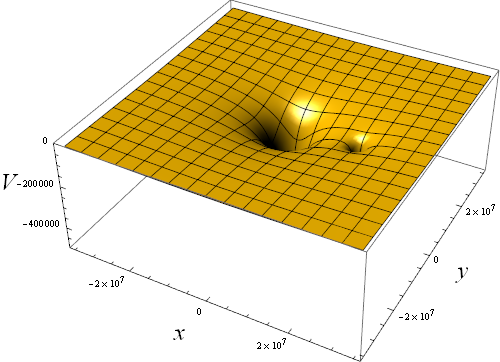
\includegraphics[scale=0.27]{pluto-charon-inertial-potential.png}}
In other words, the change in position is the velocity, and the change in
momentum (the force) is in the direction which decreases the potential.
It helps to visualise the potential for a two-dimensional problem, where the
position of a body $j$ is given by $x_j$ and $y_j$. One can plot the potential
$V\of{x_j, y_j}$ as a hilly landscape, where wells are created by the other
bodies. The force on $j$ (the change in its momentum) is then directed downhill
and its magnitude is proportional to the slope of the hill, as if $j$ were a
ball rolling atop those hills.
See for instance the potential created by Pluto and Charon in the margin.
A one-dimensional example can be seen at \url{https://xkcd.com/681_large/}.

From this formulation of the equation of motions, it is possible to deduce
properties of the trajectories just from the initial energy, even when the
trajectories are very convoluted. Indeed, since the energy is conserved and
since the kinetic energy (equal to $\frac12 m_j v_j^2$ for each body $j$)
is never negative (at worst it is $0$ for an unmoving body), the system
cannot reach a position $\vq$ where the potential $V\of\vq$ is greater than the
initial energy.

Again, this is best seen on a 2-dimensional example with a single body moving
in a fixed potential. If we plot the landscape of the potential, and a waterline
at the level of the initial energy, we know that the body cannot be found on dry
land at any time, no matter how complicated its trajectory is; if the trajectory
converts the whole of the body's kinetic energy into potential energy, it will
only reach the shore.

Moreover, the body cannot\footnote{In quantum mechanics this happens: this is
quantum tunnelling.} ``jump'' over dry land, as that would require going through
areas of potential higher than the total energy. It is confined to the ``lake''
in which it started.

The plots below show various regions allowed by the total energy in the
previously shown potential, together with example trajectories at these
energies. Note that the trajectories are computed assuming the potential is
constant (which is not true in the case of Pluto and Charon, since these bodies
revolve around each other). We'll look at a more realistic situation in a later
post.
\begin{figure}
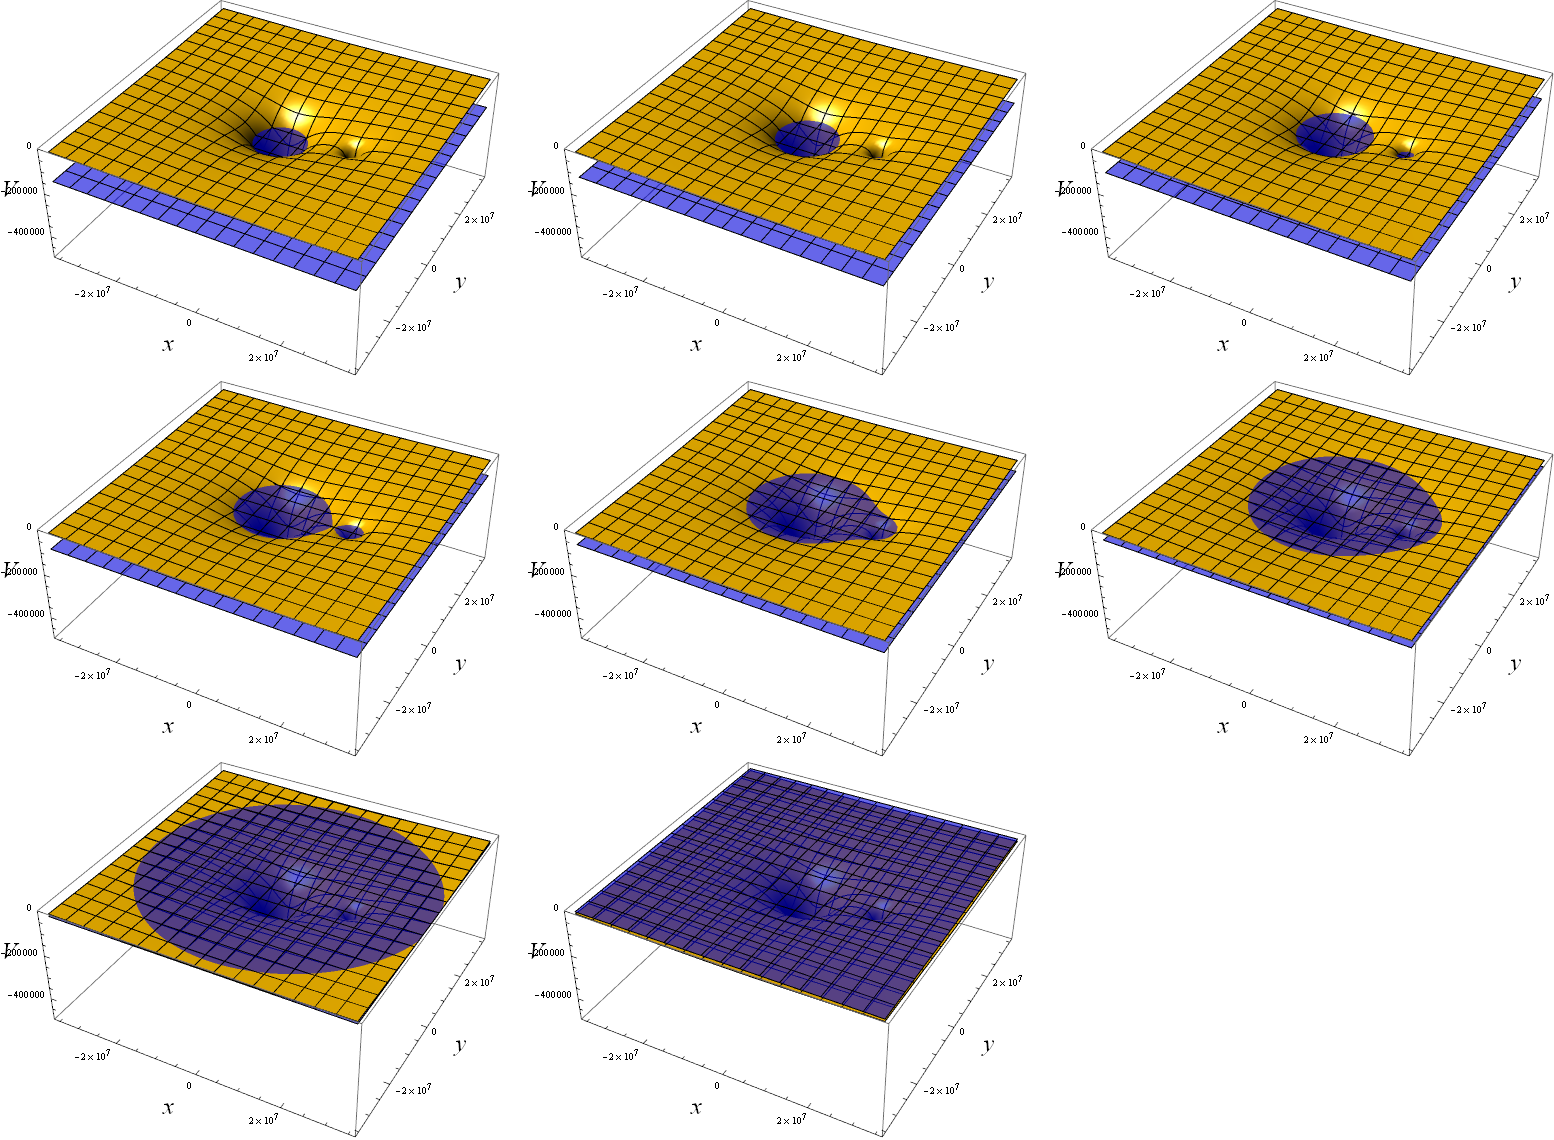
\includegraphics[scale=0.40]{rising-energy.png}
\caption{Forbidden regions (due to potential higher than the initial energy) for
various initial energies, with example trajectories. The energy of the body is
the blue plane, the potential is the yellow surface.}
\end{figure}

\section{Generalised coordinates}
We will now look at another strength of the Hamiltonian formulation of classical
mechanics: it allows for the use of coordinate systems more appropriate to the
problem at hand.

Consider a pendulum made of a point mass $m$ suspended in a vacuum with a
massless rod of length $r$ from a frictionless hinge\footnote{We will not be
needing the spherical cows today.}, under the influence of uniform standard
gravity $g_0$.
\marginfig[A mathematical pendulum.]{\FigureSimplePendulumConfigurationSpace}

At first glance, this may seem like a 2-dimensional problem since the pendulum
does not move in a straight line. However, since the pendulum is restricted by
the rod to a circle around the pivot, we can describe its position uniquely by
the oriented angle $\gq$ between the rod and the vertical: we shall use this as
our \emph{generalised position}.

Lagrangian mechanics, which is beyond the scope of this overview, is needed to
derive the corresponding generalised momentum. We shall take for granted
that this is the angular momentum $L = mr^2\gw$, where $\gw = \deriv t\gq$ is
the angular velocity.

Our state $\tuple{\gq, L}$ thus lies in a 2-dimensonial phase space. We can
now compute the Hamiltonian. The kinetic energy of our mass is
\[T = \frac{1}{2} m v^2 
    = \frac{1}{2} m \pa{r\gw}^2 
    = \frac{L^2}{2mr^2}.\]
\marginfig[The potential of the pendulum, with $m = 1\:\mathrm{kg}$ and
$r = 1\:\mathrm{m}$. $V$ in Joules, $\gq$ in radians.]{
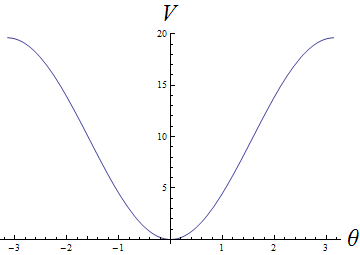
\includegraphics[scale=0.27]{pendulum-potential.png}}
The potential energy is $mg_0h$, where $h$ is the height of the mass, so we can
express it as
\[V = mg_0h = -mg_0(\cos \gq - 1).\]
We can then apply the equations of motions to that problem, and solve it as a
1-dimensional problem, using these more convenient coordinates. We will come
back to this problem in the next post to study another fundamental conservation
law related to Hamiltonian systems.

\section{Conclusion}
We see that the nature of the possible trajectories changes fundamentally when
the energy changes, from strongly-bound orbits to transfers to outright escapes.
It would therefore be useful to be able to guarantee that energy does not drift
too much even over long periods of time when numerically computing these
trajectories. Surprisingly, while guaranteeing that the actual position does not
drift away from the truth is impossible, it \emph{is} possible to ensure that the
\emph{energy} does not drift, thus ensuring that the essential nature of the
trajectory remains unchanged.

Integrators which enforce conservation of energy are called \emph{symplectic}
integrators. They rely on another property of Hamiltonian systems,
symplecticity, which will be the focus of the next post.

\end{document}